\documentclass[Report.tex]{subfiles}
\begin{document}
In this section we do Principle Component Analysis on aggregated on one season of football data. The data includes observations like the number of goals, the number of shots, the number of passings and so on. The data is collected for each player, but we have summed it to each team. We would like to find any clusters by using PCA in R.

The resulting scree plot from doing the PCA is seen in Figure \ref{fig:scree}.
\begin{figure}
\center
\includegraphics[width=\textwidth]{"scree plot".pdf}
\caption{The resulting scree plot}
\label{fig:scree}
\end{figure}
The scree plot tells us which eigenvectors have the highest eigenvalue, meaning which principle components describe the most of the data. In our case we find that the first two components describe a lot of the variance in the data, to some extend also component 3. 

\begin{figure}
\center
\includegraphics[width=\textwidth]{"PC1 Loadings".pdf}
\caption{Loadings for PC1}
\label{fig:PC1Loadings}
\end{figure}
We know look at the loadings each of the components that we choose to keep. The loadings describe the importance of the different variables in relation to the chosen component. In Figure \ref{fig:PC1Loadings} we see the loadings for PC1. Being that PC1 is the component describing most of the variance in the data, the most important variables of PC1 is also the most important variables for the entire data set. The five most important variables in regards to PC1 is the "Sum.of.Chances", "Sum.of.2nd.Assist.To.Shot", "Sum.of.Fouls.Received.In.Second.Third.Part", "Sum.of.Assist.To.Goal" and "Sum.of.Shots.On.Target".

\begin{figure}
\center
\includegraphics[width=0.49\textwidth]{"PC2 Loadings".pdf}
\includegraphics[width=0.49\textwidth]{"PC3 Loadings".pdf}
\caption{Loadings for PC2 and PC3}
\label{fig:PC23Loadings}
\end{figure}

We can do the same with PC2 and PC3. These are seen at Figure \ref{fig:PC23Loadings}. From the loadings in regard to PC2 we conclude that the five most important variables are the "Sum.of.50.50.Air.Challenges", "Sum.of.50.50.Air.Challenges.Won", "Sum.of.Crosses.On.Restart.Of.Play", "Sum.of.Successful.Crosses" and "Sum.of.Crosses".
For PC3 the five most important variables are the "Sum.of.Fouls.Received.In.First.Third.Part", "Sum.of.Goals.With.Right.Foot", "Sum.of.Tackles.Made.Won", "Sum.of.Goals.With.Foot" and "Sum.of.Crosses.In.Game".


We can now plot the data points in regards to the principle components to find clusters. The data is sorted in regards to current position of the teams in the table. This means that we easily can find out if the top/bottom teams cluster. In Figure \ref{fig:PC12} the data is plotted in regard to PC1 and PC2. We do not have any clear clusterings, some teams are clustered in the middle but there is no correlation between the standings and the teams clustering.

\begin{figure}
\center
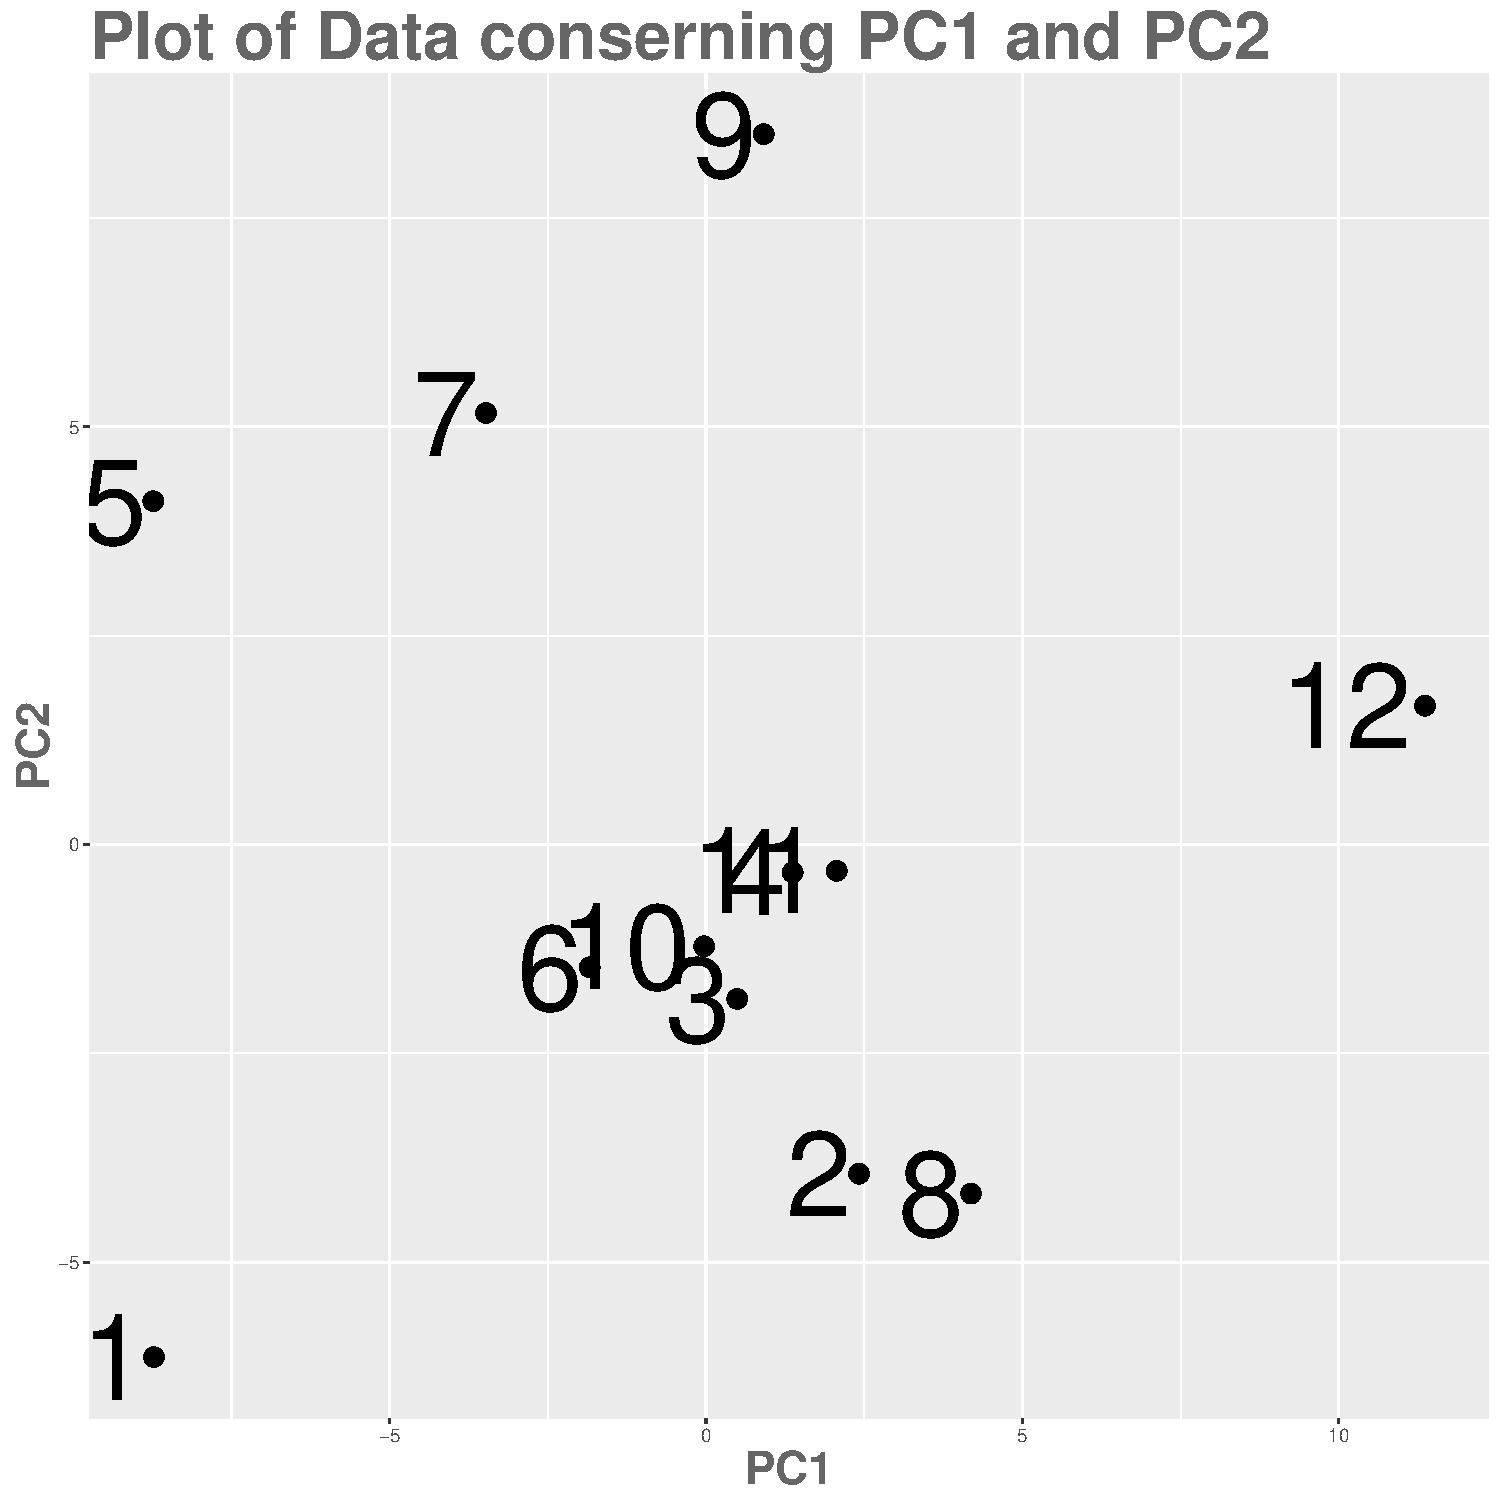
\includegraphics[scale=0.4]{PC12.pdf}
\caption{The data plotted in regard to PC1 and PC2}
\label{fig:PC12}
\end{figure}
In Figure \ref{fig:PC23} the data is plotted in regard to PC2 and PC3. Once again we have a little cluster, but there is no relation to the standings.

The PCA has not giving any clusters, but it has giving us some of the most important variables of the dataset. 

\begin{figure}
\center
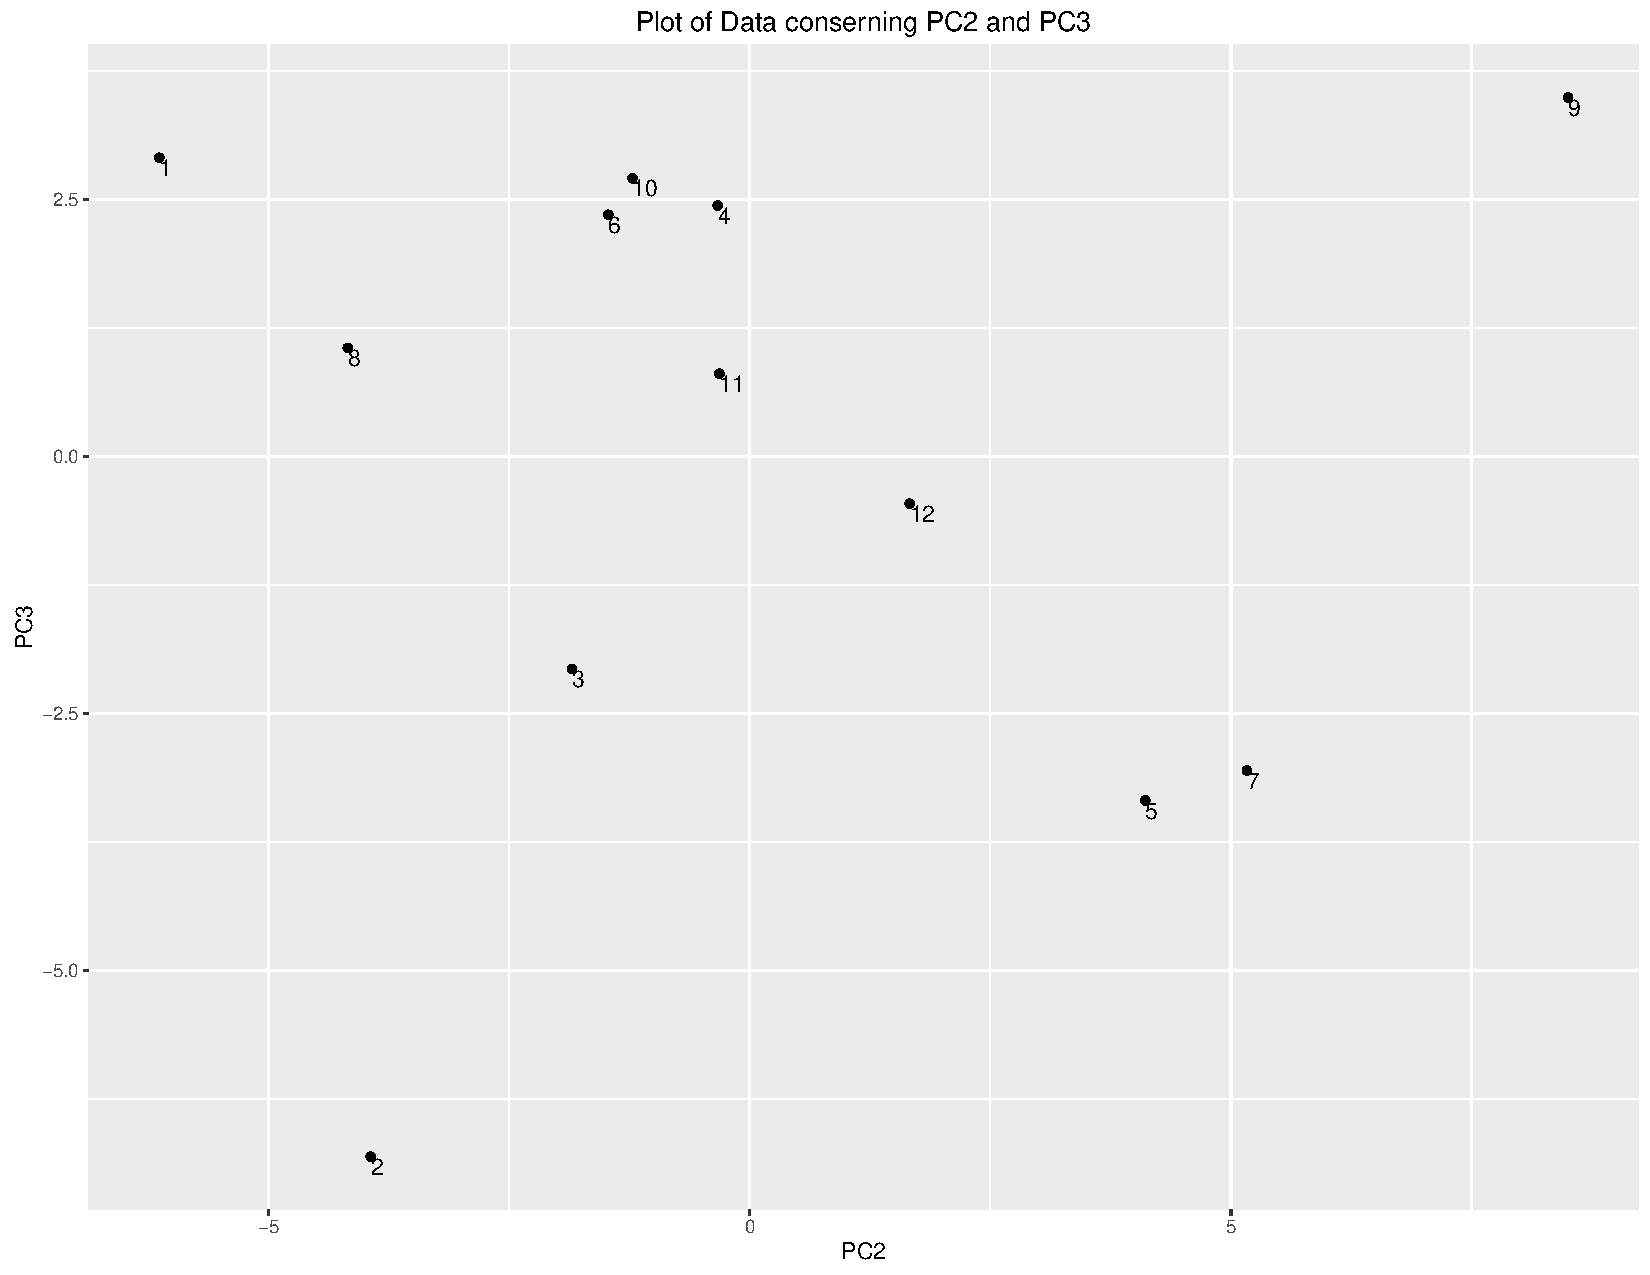
\includegraphics[scale=0.4]{PC23.pdf}
\caption{The data plotted in regard to PC2 and PC3}
\label{fig:PC23}
\end{figure}


\end{document}